\documentclass[twoside]{book}

% Packages required by doxygen
\usepackage{fixltx2e}
\usepackage{calc}
\usepackage{doxygen}
\usepackage[export]{adjustbox} % also loads graphicx
\usepackage{graphicx}
\usepackage[utf8]{inputenc}
\usepackage{makeidx}
\usepackage{multicol}
\usepackage{multirow}
\PassOptionsToPackage{warn}{textcomp}
\usepackage{textcomp}
\usepackage[nointegrals]{wasysym}
\usepackage[table]{xcolor}

% Font selection
\usepackage[T1]{fontenc}
\usepackage[scaled=.90]{helvet}
\usepackage{courier}
\usepackage{amssymb}
\usepackage{sectsty}
\renewcommand{\familydefault}{\sfdefault}
\allsectionsfont{%
  \fontseries{bc}\selectfont%
  \color{darkgray}%
}
\renewcommand{\DoxyLabelFont}{%
  \fontseries{bc}\selectfont%
  \color{darkgray}%
}
\newcommand{\+}{\discretionary{\mbox{\scriptsize$\hookleftarrow$}}{}{}}

% Page & text layout
\usepackage{geometry}
\geometry{%
  a4paper,%
  top=2.5cm,%
  bottom=2.5cm,%
  left=2.5cm,%
  right=2.5cm%
}
\tolerance=750
\hfuzz=15pt
\hbadness=750
\setlength{\emergencystretch}{15pt}
\setlength{\parindent}{0cm}
\setlength{\parskip}{3ex plus 2ex minus 2ex}
\makeatletter
\renewcommand{\paragraph}{%
  \@startsection{paragraph}{4}{0ex}{-1.0ex}{1.0ex}{%
    \normalfont\normalsize\bfseries\SS@parafont%
  }%
}
\renewcommand{\subparagraph}{%
  \@startsection{subparagraph}{5}{0ex}{-1.0ex}{1.0ex}{%
    \normalfont\normalsize\bfseries\SS@subparafont%
  }%
}
\makeatother

% Headers & footers
\usepackage{fancyhdr}
\pagestyle{fancyplain}
\fancyhead[LE]{\fancyplain{}{\bfseries\thepage}}
\fancyhead[CE]{\fancyplain{}{}}
\fancyhead[RE]{\fancyplain{}{\bfseries\leftmark}}
\fancyhead[LO]{\fancyplain{}{\bfseries\rightmark}}
\fancyhead[CO]{\fancyplain{}{}}
\fancyhead[RO]{\fancyplain{}{\bfseries\thepage}}
\fancyfoot[LE]{\fancyplain{}{}}
\fancyfoot[CE]{\fancyplain{}{}}
\fancyfoot[RE]{\fancyplain{}{\bfseries\scriptsize Generated by Doxygen }}
\fancyfoot[LO]{\fancyplain{}{\bfseries\scriptsize Generated by Doxygen }}
\fancyfoot[CO]{\fancyplain{}{}}
\fancyfoot[RO]{\fancyplain{}{}}
\renewcommand{\footrulewidth}{0.4pt}
\renewcommand{\chaptermark}[1]{%
  \markboth{#1}{}%
}
\renewcommand{\sectionmark}[1]{%
  \markright{\thesection\ #1}%
}

% Indices & bibliography
\usepackage{natbib}
\usepackage[titles]{tocloft}
\setcounter{tocdepth}{3}
\setcounter{secnumdepth}{5}
\makeindex

% Hyperlinks (required, but should be loaded last)
\usepackage{ifpdf}
\ifpdf
  \usepackage[pdftex,pagebackref=true]{hyperref}
\else
  \usepackage[ps2pdf,pagebackref=true]{hyperref}
\fi
\hypersetup{%
  colorlinks=true,%
  linkcolor=blue,%
  citecolor=blue,%
  unicode%
}

% Custom commands
\newcommand{\clearemptydoublepage}{%
  \newpage{\pagestyle{empty}\cleardoublepage}%
}

\usepackage{caption}
\captionsetup{labelsep=space,justification=centering,font={bf},singlelinecheck=off,skip=4pt,position=top}

%===== C O N T E N T S =====

\begin{document}

% Titlepage & ToC
\hypersetup{pageanchor=false,
             bookmarksnumbered=true,
             pdfencoding=unicode
            }
\pagenumbering{alph}
\begin{titlepage}
\vspace*{7cm}
\begin{center}%
{\Large Simple\+Graph\+No\+Sql }\\
\vspace*{1cm}
{\large Generated by Doxygen 1.8.14}\\
\end{center}
\end{titlepage}
\clearemptydoublepage
\pagenumbering{roman}
\tableofcontents
\clearemptydoublepage
\pagenumbering{arabic}
\hypersetup{pageanchor=true}

%--- Begin generated contents ---
\chapter{Hierarchical Index}
\section{Class Hierarchy}
This inheritance list is sorted roughly, but not completely, alphabetically\+:\begin{DoxyCompactList}
\item object\begin{DoxyCompactList}
\item \contentsline{section}{db.\+DB}{\pageref{classdb_1_1_d_b}}{}
\item \contentsline{section}{menus.\+Container}{\pageref{classmenus_1_1_container}}{}
\item \contentsline{section}{Tabela.\+Cell}{\pageref{class_tabela_1_1_cell}}{}
\item \contentsline{section}{Tabela.\+Raw\+Table}{\pageref{class_tabela_1_1_raw_table}}{}
\item \contentsline{section}{Tabela.\+Table}{\pageref{class_tabela_1_1_table}}{}
\item \contentsline{section}{Trie.\+Nodo}{\pageref{class_trie_1_1_nodo}}{}
\item \contentsline{section}{Trie.\+Trie}{\pageref{class_trie_1_1_trie}}{}
\end{DoxyCompactList}
\end{DoxyCompactList}

\chapter{Class Index}
\section{Class List}
Here are the classes, structs, unions and interfaces with brief descriptions\+:\begin{DoxyCompactList}
\item\contentsline{section}{\mbox{\hyperlink{class_tabela_1_1_cell}{Tabela.\+Cell}} }{\pageref{class_tabela_1_1_cell}}{}
\item\contentsline{section}{\mbox{\hyperlink{classmenus_1_1_container}{menus.\+Container}} }{\pageref{classmenus_1_1_container}}{}
\item\contentsline{section}{\mbox{\hyperlink{classdb_1_1_d_b}{db.\+DB}} }{\pageref{classdb_1_1_d_b}}{}
\item\contentsline{section}{\mbox{\hyperlink{class_trie_1_1_nodo}{Trie.\+Nodo}} }{\pageref{class_trie_1_1_nodo}}{}
\item\contentsline{section}{\mbox{\hyperlink{class_tabela_1_1_raw_table}{Tabela.\+Raw\+Table}} }{\pageref{class_tabela_1_1_raw_table}}{}
\item\contentsline{section}{\mbox{\hyperlink{class_tabela_1_1_table}{Tabela.\+Table}} }{\pageref{class_tabela_1_1_table}}{}
\item\contentsline{section}{\mbox{\hyperlink{class_trie_1_1_trie}{Trie.\+Trie}} }{\pageref{class_trie_1_1_trie}}{}
\end{DoxyCompactList}

\chapter{Class Documentation}
\hypertarget{class_tabela_1_1_cell}{}\section{Tabela.\+Cell Class Reference}
\label{class_tabela_1_1_cell}\index{Tabela.\+Cell@{Tabela.\+Cell}}
Inheritance diagram for Tabela.\+Cell\+:\begin{figure}[H]
\begin{center}
\leavevmode
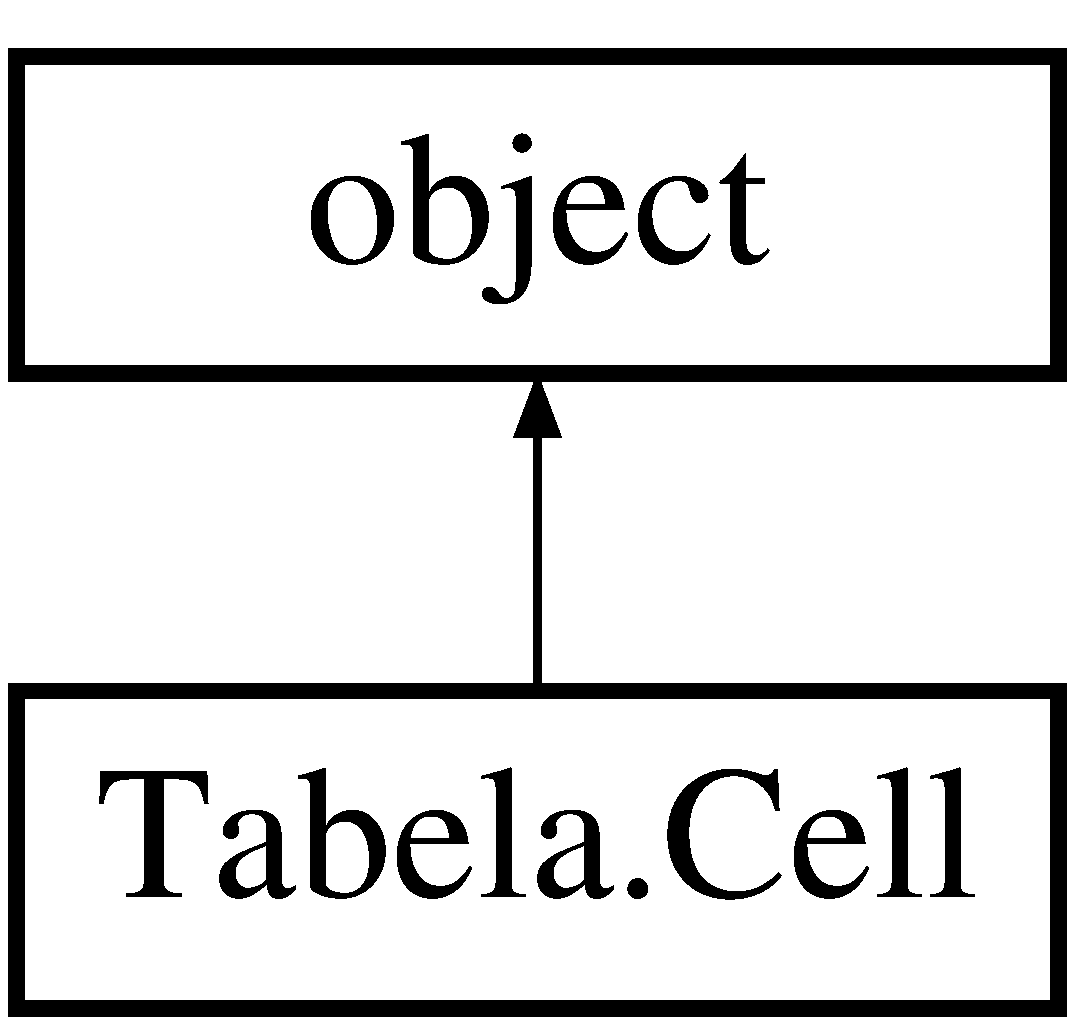
\includegraphics[height=2.000000cm]{class_tabela_1_1_cell}
\end{center}
\end{figure}
\subsection*{Public Member Functions}
\begin{DoxyCompactItemize}
\item 
\mbox{\Hypertarget{class_tabela_1_1_cell_a0cc729a89011b7ebd701ca6f1405f122}\label{class_tabela_1_1_cell_a0cc729a89011b7ebd701ca6f1405f122}} 
def {\bfseries \+\_\+\+\_\+init\+\_\+\+\_\+} (self, sheet, X, Y)
\end{DoxyCompactItemize}
\subsection*{Public Attributes}
\begin{DoxyCompactItemize}
\item 
\mbox{\hyperlink{class_tabela_1_1_cell_a81d6743175d93342642a052894df99a2}{data\+\_\+boundary}}
\begin{DoxyCompactList}\small\item\em Inicializa celula, definindo atribuitos e o tipo da celula self.\+cell\+\_\+type define o tipo da variavel\+: Tipos possiveis\+: Leaf -\/$>$ Representa uma celula do excel contendo dados e mais nada. \end{DoxyCompactList}\item 
\mbox{\Hypertarget{class_tabela_1_1_cell_a595c89589e45916787b38d9bbcf41bf7}\label{class_tabela_1_1_cell_a595c89589e45916787b38d9bbcf41bf7}} 
{\bfseries blank\+\_\+boundary}
\item 
\mbox{\Hypertarget{class_tabela_1_1_cell_a543900af4f49d7f7dce5be24aaddcd43}\label{class_tabela_1_1_cell_a543900af4f49d7f7dce5be24aaddcd43}} 
{\bfseries originx}
\item 
\mbox{\Hypertarget{class_tabela_1_1_cell_ac06d52d26c63f8b64c206f3a090bf91b}\label{class_tabela_1_1_cell_ac06d52d26c63f8b64c206f3a090bf91b}} 
{\bfseries originy}
\item 
\mbox{\Hypertarget{class_tabela_1_1_cell_a8e5d57b52807b55546c2443470e0f85f}\label{class_tabela_1_1_cell_a8e5d57b52807b55546c2443470e0f85f}} 
{\bfseries sizex}
\item 
\mbox{\Hypertarget{class_tabela_1_1_cell_a226e9b058ada2e873243f45136b2a9ce}\label{class_tabela_1_1_cell_a226e9b058ada2e873243f45136b2a9ce}} 
{\bfseries sizey}
\item 
\mbox{\Hypertarget{class_tabela_1_1_cell_a6601b87d017e8dc40c575858bb9aefab}\label{class_tabela_1_1_cell_a6601b87d017e8dc40c575858bb9aefab}} 
{\bfseries x}
\item 
\mbox{\Hypertarget{class_tabela_1_1_cell_aec268ed0feba78f5d5affd5b1affbc67}\label{class_tabela_1_1_cell_aec268ed0feba78f5d5affd5b1affbc67}} 
{\bfseries y}
\item 
\mbox{\Hypertarget{class_tabela_1_1_cell_ad31ac1bf3ec1335d25343f113ef6a564}\label{class_tabela_1_1_cell_ad31ac1bf3ec1335d25343f113ef6a564}} 
{\bfseries bounds}
\item 
\mbox{\Hypertarget{class_tabela_1_1_cell_a822efbac3e8b7c912a2e33ce0d106c84}\label{class_tabela_1_1_cell_a822efbac3e8b7c912a2e33ce0d106c84}} 
{\bfseries cell\+\_\+type}
\item 
\mbox{\Hypertarget{class_tabela_1_1_cell_aae4fd1ac2cefbce827ff7713e6db3a52}\label{class_tabela_1_1_cell_aae4fd1ac2cefbce827ff7713e6db3a52}} 
{\bfseries data}
\item 
\mbox{\Hypertarget{class_tabela_1_1_cell_adc1415ea59c977255d5d5c9ee0235453}\label{class_tabela_1_1_cell_adc1415ea59c977255d5d5c9ee0235453}} 
{\bfseries table\+\_\+label}
\item 
\mbox{\Hypertarget{class_tabela_1_1_cell_ac37f9319e055d0ca765ba3c77d68252c}\label{class_tabela_1_1_cell_ac37f9319e055d0ca765ba3c77d68252c}} 
{\bfseries parent\+\_\+node}
\item 
\mbox{\Hypertarget{class_tabela_1_1_cell_a6c52a49677bbce958aa0b7c037892942}\label{class_tabela_1_1_cell_a6c52a49677bbce958aa0b7c037892942}} 
{\bfseries child\+\_\+nodes}
\item 
\mbox{\Hypertarget{class_tabela_1_1_cell_a9086096bb2d966a75e18722fcb2659d1}\label{class_tabela_1_1_cell_a9086096bb2d966a75e18722fcb2659d1}} 
{\bfseries key\+\_\+row}
\item 
\mbox{\Hypertarget{class_tabela_1_1_cell_a9d9b117373e9ddef7a2ad8832d4da842}\label{class_tabela_1_1_cell_a9d9b117373e9ddef7a2ad8832d4da842}} 
{\bfseries key\+\_\+col}
\item 
\mbox{\Hypertarget{class_tabela_1_1_cell_a54bfaf35d099a9c6bd88a032618a2528}\label{class_tabela_1_1_cell_a54bfaf35d099a9c6bd88a032618a2528}} 
{\bfseries cell\+\_\+name}
\end{DoxyCompactItemize}


\subsection{Detailed Description}
\begin{DoxyVerb}Classe que representa uma celula da tabela. Recebe um objeto do tipo sheet do xrld como entrada
    e uma posicao X referente a linha e Y referente a celula. Cria um objeto do tipo celula classificando o tipo de celula e guardando dados\end{DoxyVerb}
 

\subsection{Member Data Documentation}
\mbox{\Hypertarget{class_tabela_1_1_cell_a81d6743175d93342642a052894df99a2}\label{class_tabela_1_1_cell_a81d6743175d93342642a052894df99a2}} 
\index{Tabela\+::\+Cell@{Tabela\+::\+Cell}!data\+\_\+boundary@{data\+\_\+boundary}}
\index{data\+\_\+boundary@{data\+\_\+boundary}!Tabela\+::\+Cell@{Tabela\+::\+Cell}}
\subsubsection{\texorpdfstring{data\+\_\+boundary}{data\_boundary}}
{\footnotesize\ttfamily Tabela.\+Cell.\+data\+\_\+boundary}



Inicializa celula, definindo atribuitos e o tipo da celula self.\+cell\+\_\+type define o tipo da variavel\+: Tipos possiveis\+: Leaf -\/$>$ Representa uma celula do excel contendo dados e mais nada. 

É relacionada a duas chaves, uma de linha(key) e outra de coluna(key\+\_\+col) \+: Key\+\_\+\+Row -\/$>$ Representa uma chave que ordena outras chaves(exemplo\+: A\+N\+O). Uma por tabela Key\+\_\+\+Col -\/$>$Representa uma chave que dá sentido a uma coluna. Podem existir varias por tabela Key -\/$>$ Representa uma chave presente em uma Key\+\_\+col Super\+\_\+\+Key -\/$>$ Representa uma chave que é pai de outras chaves ou de uma chave coluna. Label -\/$>$ Representa o nome da tabela, é a raiz da arvore e pai de todos os outros nodos Merge -\/$>$ Representa uma celula que foi unida uma outra celula e não tem dados Blank -\/$>$Não faz parte da tabela, dado vazio que pode ser removido sem alterações 

The documentation for this class was generated from the following file\+:\begin{DoxyCompactItemize}
\item 
C\+:/\+Users/\+P\+C/source/repos/\+Trabalho\+\_\+final\+\_\+cpd/\+Simple\+Graph\+No\+S\+Q\+L/Tabela.\+py\end{DoxyCompactItemize}

\hypertarget{classmenus_1_1_container}{}\section{menus.\+Container Class Reference}
\label{classmenus_1_1_container}\index{menus.\+Container@{menus.\+Container}}
Inheritance diagram for menus.\+Container\+:\begin{figure}[H]
\begin{center}
\leavevmode
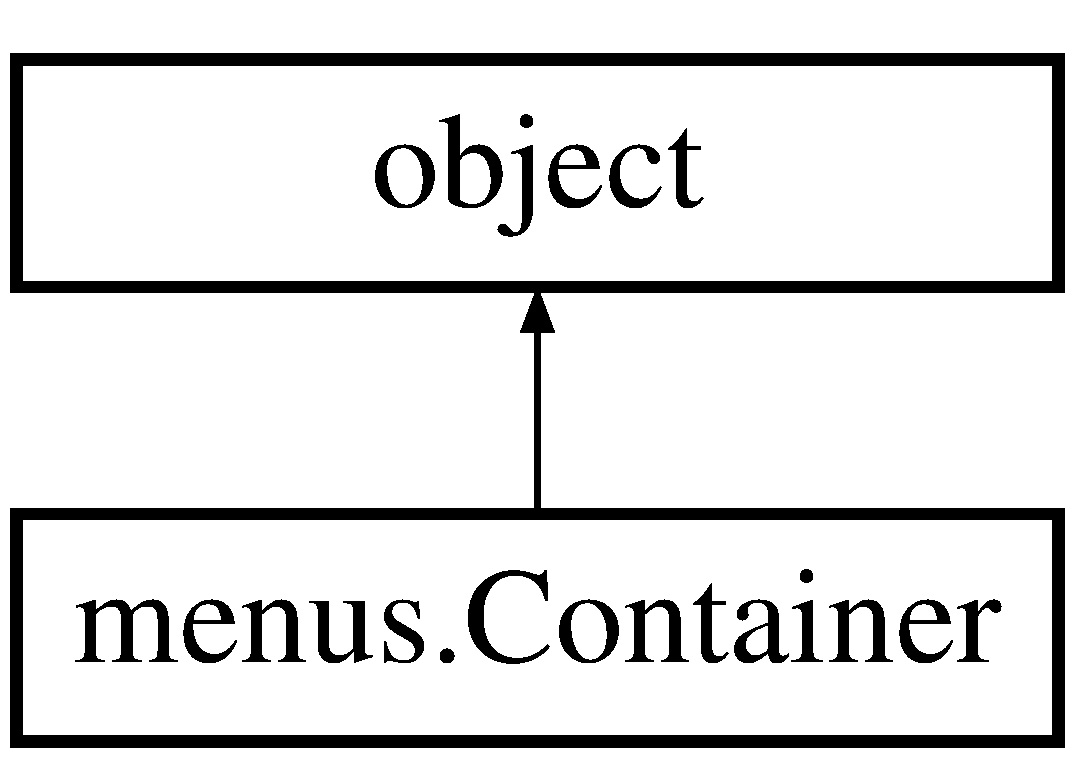
\includegraphics[height=2.000000cm]{classmenus_1_1_container}
\end{center}
\end{figure}
\subsection*{Public Member Functions}
\begin{DoxyCompactItemize}
\item 
\mbox{\Hypertarget{classmenus_1_1_container_ace093b51d065a19a56b39467aa1cfe66}\label{classmenus_1_1_container_ace093b51d065a19a56b39467aa1cfe66}} 
def {\bfseries \+\_\+\+\_\+init\+\_\+\+\_\+} (self, data)
\end{DoxyCompactItemize}
\subsection*{Public Attributes}
\begin{DoxyCompactItemize}
\item 
\mbox{\Hypertarget{classmenus_1_1_container_ac6d2c5aabad726f4fe51f22f96c3f12e}\label{classmenus_1_1_container_ac6d2c5aabad726f4fe51f22f96c3f12e}} 
{\bfseries raw\+\_\+type}
\item 
\mbox{\Hypertarget{classmenus_1_1_container_a926a48b4cde967e8ca8c394abc09e690}\label{classmenus_1_1_container_a926a48b4cde967e8ca8c394abc09e690}} 
{\bfseries name}
\item 
\mbox{\Hypertarget{classmenus_1_1_container_ace4ff1a1c445f0bba0026fbc3df35f63}\label{classmenus_1_1_container_ace4ff1a1c445f0bba0026fbc3df35f63}} 
{\bfseries data}
\item 
\mbox{\Hypertarget{classmenus_1_1_container_a96af1c60b4ea020510e940361a0008c9}\label{classmenus_1_1_container_a96af1c60b4ea020510e940361a0008c9}} 
{\bfseries type}
\end{DoxyCompactItemize}


\subsection{Detailed Description}
\begin{DoxyVerb}Classe representando um objeto que pode ser um Nodo ou uma Tabela ou uma Lista de celulas ou uma Celula. data representa o objeto a gerar o container
\end{DoxyVerb}
 

The documentation for this class was generated from the following file\+:\begin{DoxyCompactItemize}
\item 
C\+:/\+Users/\+P\+C/source/repos/\+Trabalho\+\_\+final\+\_\+cpd/\+Simple\+Graph\+No\+S\+Q\+L/menus.\+py\end{DoxyCompactItemize}

\hypertarget{classdb_1_1_d_b}{}\section{db.\+DB Class Reference}
\label{classdb_1_1_d_b}\index{db.\+DB@{db.\+DB}}
Inheritance diagram for db.\+DB\+:\begin{figure}[H]
\begin{center}
\leavevmode
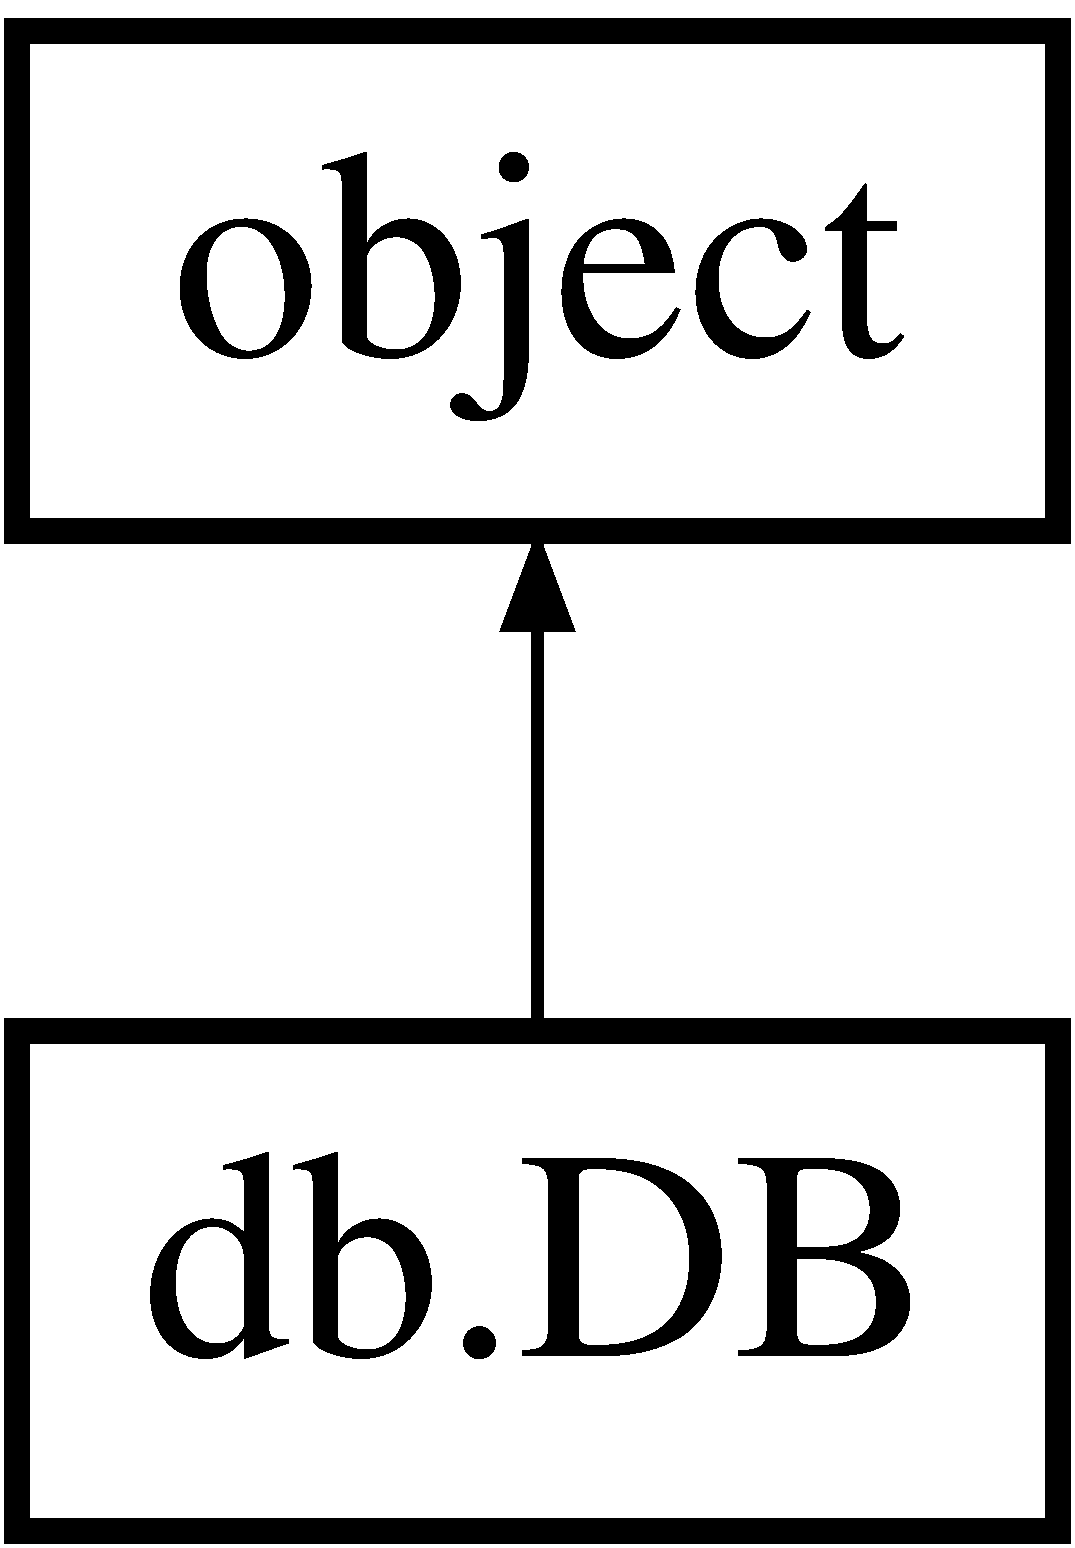
\includegraphics[height=2.000000cm]{classdb_1_1_d_b}
\end{center}
\end{figure}
\subsection*{Public Member Functions}
\begin{DoxyCompactItemize}
\item 
def \mbox{\hyperlink{classdb_1_1_d_b_af1e6dda03c0f1c1a5bf4b993865a5b3a}{\+\_\+\+\_\+init\+\_\+\+\_\+}} (self, trie)
\end{DoxyCompactItemize}
\subsection*{Public Attributes}
\begin{DoxyCompactItemize}
\item 
\mbox{\Hypertarget{classdb_1_1_d_b_afa64c6cf6218f2423e0894a5cf0102bb}\label{classdb_1_1_d_b_afa64c6cf6218f2423e0894a5cf0102bb}} 
{\bfseries tables}
\item 
\mbox{\Hypertarget{classdb_1_1_d_b_a5993ee8357b3bb993484d83a98a8b828}\label{classdb_1_1_d_b_a5993ee8357b3bb993484d83a98a8b828}} 
{\bfseries key\+\_\+rows}
\item 
\mbox{\Hypertarget{classdb_1_1_d_b_ad162712835b5eb50f3cce0bfd39ba244}\label{classdb_1_1_d_b_ad162712835b5eb50f3cce0bfd39ba244}} 
{\bfseries key\+\_\+cols}
\item 
\mbox{\Hypertarget{classdb_1_1_d_b_a47d36e897b9f59edde9fdc23e0d9a5f0}\label{classdb_1_1_d_b_a47d36e897b9f59edde9fdc23e0d9a5f0}} 
{\bfseries super\+\_\+key}
\end{DoxyCompactItemize}


\subsection{Detailed Description}
\begin{DoxyVerb}Cria banco de dados a partir de uma trie de tabelas\end{DoxyVerb}
 

\subsection{Constructor \& Destructor Documentation}
\mbox{\Hypertarget{classdb_1_1_d_b_af1e6dda03c0f1c1a5bf4b993865a5b3a}\label{classdb_1_1_d_b_af1e6dda03c0f1c1a5bf4b993865a5b3a}} 
\index{db\+::\+DB@{db\+::\+DB}!\+\_\+\+\_\+init\+\_\+\+\_\+@{\+\_\+\+\_\+init\+\_\+\+\_\+}}
\index{\+\_\+\+\_\+init\+\_\+\+\_\+@{\+\_\+\+\_\+init\+\_\+\+\_\+}!db\+::\+DB@{db\+::\+DB}}
\subsubsection{\texorpdfstring{\+\_\+\+\_\+init\+\_\+\+\_\+()}{\_\_init\_\_()}}
{\footnotesize\ttfamily def db.\+D\+B.\+\_\+\+\_\+init\+\_\+\+\_\+ (\begin{DoxyParamCaption}\item[{}]{self,  }\item[{}]{trie }\end{DoxyParamCaption})}

\begin{DoxyVerb}Inicialize banco de dados com uma trie recebida\end{DoxyVerb}
 

The documentation for this class was generated from the following file\+:\begin{DoxyCompactItemize}
\item 
C\+:/\+Users/\+P\+C/source/repos/\+Trabalho\+\_\+final\+\_\+cpd/\+Simple\+Graph\+No\+S\+Q\+L/db.\+py\end{DoxyCompactItemize}

\hypertarget{class_trie_1_1_nodo}{}\section{Trie.\+Nodo Class Reference}
\label{class_trie_1_1_nodo}\index{Trie.\+Nodo@{Trie.\+Nodo}}
Inheritance diagram for Trie.\+Nodo\+:\begin{figure}[H]
\begin{center}
\leavevmode
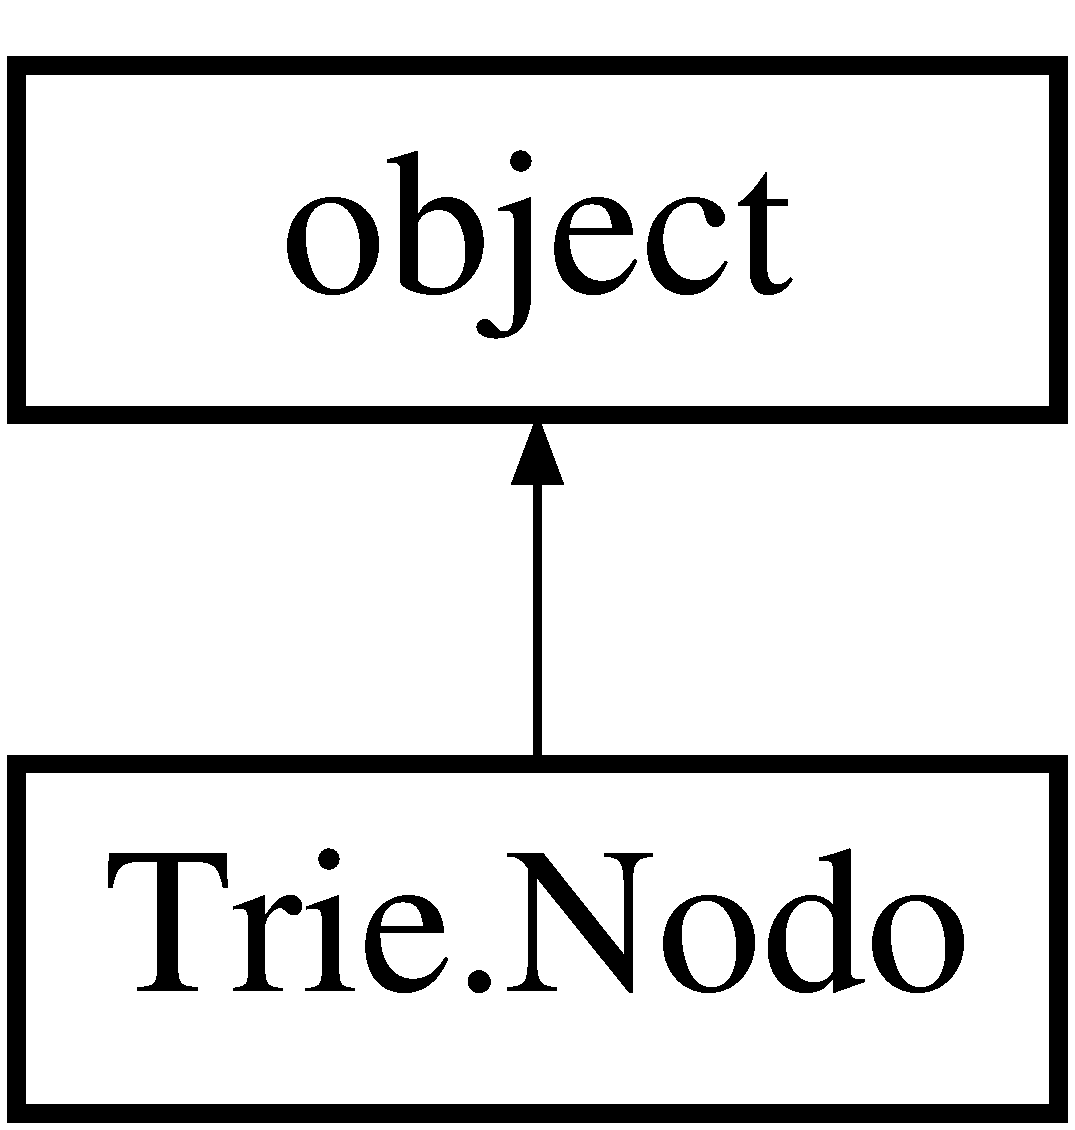
\includegraphics[height=2.000000cm]{class_trie_1_1_nodo}
\end{center}
\end{figure}
\subsection*{Public Member Functions}
\begin{DoxyCompactItemize}
\item 
def \mbox{\hyperlink{class_trie_1_1_nodo_a14edf9313e0cb711a55c47d8250b566b}{\+\_\+\+\_\+init\+\_\+\+\_\+}} (self, char\+\_\+data, data)
\end{DoxyCompactItemize}
\subsection*{Public Attributes}
\begin{DoxyCompactItemize}
\item 
\mbox{\Hypertarget{class_trie_1_1_nodo_a4d02f803001c14b673ec515096536cf5}\label{class_trie_1_1_nodo_a4d02f803001c14b673ec515096536cf5}} 
{\bfseries child}
\item 
\mbox{\Hypertarget{class_trie_1_1_nodo_a554b24962e680d0641df132499788c01}\label{class_trie_1_1_nodo_a554b24962e680d0641df132499788c01}} 
{\bfseries parent}
\item 
\mbox{\Hypertarget{class_trie_1_1_nodo_ac3ea66bba593e72a8b0db4b7b70c48a9}\label{class_trie_1_1_nodo_ac3ea66bba593e72a8b0db4b7b70c48a9}} 
{\bfseries chard}
\item 
\mbox{\Hypertarget{class_trie_1_1_nodo_ad96070f8122b253194611b8f8b0d4e86}\label{class_trie_1_1_nodo_ad96070f8122b253194611b8f8b0d4e86}} 
{\bfseries data}
\end{DoxyCompactItemize}


\subsection{Detailed Description}
\begin{DoxyVerb}Representa um nodo de uma trie\end{DoxyVerb}
 

\subsection{Constructor \& Destructor Documentation}
\mbox{\Hypertarget{class_trie_1_1_nodo_a14edf9313e0cb711a55c47d8250b566b}\label{class_trie_1_1_nodo_a14edf9313e0cb711a55c47d8250b566b}} 
\index{Trie\+::\+Nodo@{Trie\+::\+Nodo}!\+\_\+\+\_\+init\+\_\+\+\_\+@{\+\_\+\+\_\+init\+\_\+\+\_\+}}
\index{\+\_\+\+\_\+init\+\_\+\+\_\+@{\+\_\+\+\_\+init\+\_\+\+\_\+}!Trie\+::\+Nodo@{Trie\+::\+Nodo}}
\subsubsection{\texorpdfstring{\+\_\+\+\_\+init\+\_\+\+\_\+()}{\_\_init\_\_()}}
{\footnotesize\ttfamily def Trie.\+Nodo.\+\_\+\+\_\+init\+\_\+\+\_\+ (\begin{DoxyParamCaption}\item[{}]{self,  }\item[{}]{char\+\_\+data,  }\item[{}]{data }\end{DoxyParamCaption})}

\begin{DoxyVerb}Inicializa nodos com dados. char_data é o caractere, e data são os dados ligados aquele nodo. Representar nenhum dado como 0 \end{DoxyVerb}
 

The documentation for this class was generated from the following file\+:\begin{DoxyCompactItemize}
\item 
C\+:/\+Users/\+P\+C/source/repos/\+Trabalho\+\_\+final\+\_\+cpd/\+Simple\+Graph\+No\+S\+Q\+L/Trie.\+py\end{DoxyCompactItemize}

\hypertarget{class_tabela_1_1_raw_table}{}\section{Tabela.\+Raw\+Table Class Reference}
\label{class_tabela_1_1_raw_table}\index{Tabela.\+Raw\+Table@{Tabela.\+Raw\+Table}}
Inheritance diagram for Tabela.\+Raw\+Table\+:\begin{figure}[H]
\begin{center}
\leavevmode
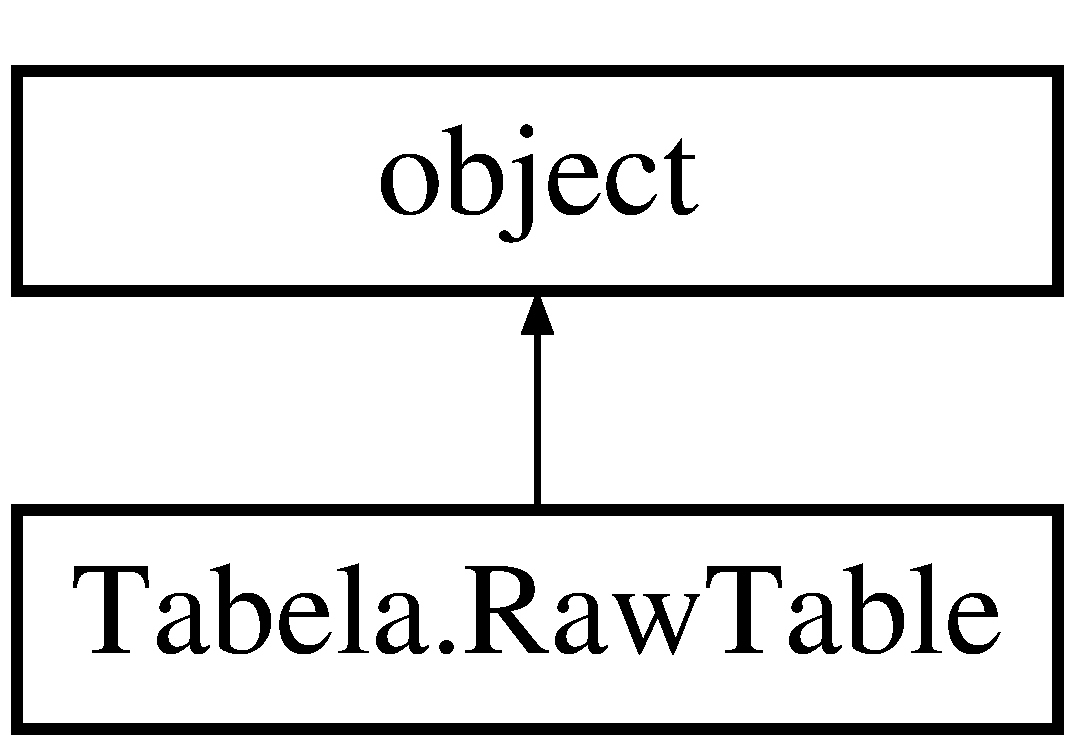
\includegraphics[height=2.000000cm]{class_tabela_1_1_raw_table}
\end{center}
\end{figure}
\subsection*{Public Member Functions}
\begin{DoxyCompactItemize}
\item 
def \mbox{\hyperlink{class_tabela_1_1_raw_table_afceb720336b1c4ac7084cfc2719514fa}{\+\_\+\+\_\+init\+\_\+\+\_\+}} (self, loc)
\end{DoxyCompactItemize}
\subsection*{Public Attributes}
\begin{DoxyCompactItemize}
\item 
\mbox{\Hypertarget{class_tabela_1_1_raw_table_a8c34690e14cf866b1477a88cee953ce5}\label{class_tabela_1_1_raw_table_a8c34690e14cf866b1477a88cee953ce5}} 
{\bfseries loc\+\_\+source}
\item 
\mbox{\Hypertarget{class_tabela_1_1_raw_table_a2e27d60b90222e80510e3d39b6856142}\label{class_tabela_1_1_raw_table_a2e27d60b90222e80510e3d39b6856142}} 
{\bfseries raw\+\_\+table}
\item 
\mbox{\Hypertarget{class_tabela_1_1_raw_table_ad954dccabbbdbd2616c4e48620a5b121}\label{class_tabela_1_1_raw_table_ad954dccabbbdbd2616c4e48620a5b121}} 
{\bfseries raw\+\_\+sheet}
\item 
\mbox{\Hypertarget{class_tabela_1_1_raw_table_a31c6abc84cf6f1fb1df2e9b14406746e}\label{class_tabela_1_1_raw_table_a31c6abc84cf6f1fb1df2e9b14406746e}} 
{\bfseries table\+\_\+label}
\item 
\mbox{\Hypertarget{class_tabela_1_1_raw_table_a47a68a2235c0bafa906cd122db44cb85}\label{class_tabela_1_1_raw_table_a47a68a2235c0bafa906cd122db44cb85}} 
{\bfseries table\+\_\+data}
\item 
\mbox{\Hypertarget{class_tabela_1_1_raw_table_a2d905e086c422c2cc296c60d4c4e729b}\label{class_tabela_1_1_raw_table_a2d905e086c422c2cc296c60d4c4e729b}} 
{\bfseries bound\+\_\+x}
\item 
\mbox{\Hypertarget{class_tabela_1_1_raw_table_af4c910628f1271516d6cba7b5117c0f5}\label{class_tabela_1_1_raw_table_af4c910628f1271516d6cba7b5117c0f5}} 
{\bfseries bound\+\_\+y}
\item 
\mbox{\Hypertarget{class_tabela_1_1_raw_table_a9298050415197ab6c56c409107676362}\label{class_tabela_1_1_raw_table_a9298050415197ab6c56c409107676362}} 
{\bfseries key\+\_\+cols}
\item 
\mbox{\Hypertarget{class_tabela_1_1_raw_table_aadade37b733a5ffeacfa6afd63247124}\label{class_tabela_1_1_raw_table_aadade37b733a5ffeacfa6afd63247124}} 
{\bfseries key\+\_\+row}
\item 
\mbox{\Hypertarget{class_tabela_1_1_raw_table_a10fc3b2dcf218f5121d2688869889d8c}\label{class_tabela_1_1_raw_table_a10fc3b2dcf218f5121d2688869889d8c}} 
{\bfseries keys}
\end{DoxyCompactItemize}


\subsection{Detailed Description}
\begin{DoxyVerb}Classe que representa uma tabela do excel na memoria. Guarda mais dados do que o necessario e não consegue ser pickleada\end{DoxyVerb}
 

\subsection{Constructor \& Destructor Documentation}
\mbox{\Hypertarget{class_tabela_1_1_raw_table_afceb720336b1c4ac7084cfc2719514fa}\label{class_tabela_1_1_raw_table_afceb720336b1c4ac7084cfc2719514fa}} 
\index{Tabela\+::\+Raw\+Table@{Tabela\+::\+Raw\+Table}!\+\_\+\+\_\+init\+\_\+\+\_\+@{\+\_\+\+\_\+init\+\_\+\+\_\+}}
\index{\+\_\+\+\_\+init\+\_\+\+\_\+@{\+\_\+\+\_\+init\+\_\+\+\_\+}!Tabela\+::\+Raw\+Table@{Tabela\+::\+Raw\+Table}}
\subsubsection{\texorpdfstring{\+\_\+\+\_\+init\+\_\+\+\_\+()}{\_\_init\_\_()}}
{\footnotesize\ttfamily def Tabela.\+Raw\+Table.\+\_\+\+\_\+init\+\_\+\+\_\+ (\begin{DoxyParamCaption}\item[{}]{self,  }\item[{}]{loc }\end{DoxyParamCaption})}

\begin{DoxyVerb}Inicializa uma tabela a partir de um local loc\end{DoxyVerb}
 

The documentation for this class was generated from the following file\+:\begin{DoxyCompactItemize}
\item 
C\+:/\+Users/\+P\+C/source/repos/\+Trabalho\+\_\+final\+\_\+cpd/\+Simple\+Graph\+No\+S\+Q\+L/Tabela.\+py\end{DoxyCompactItemize}

\hypertarget{class_tabela_1_1_table}{}\section{Tabela.\+Table Class Reference}
\label{class_tabela_1_1_table}\index{Tabela.\+Table@{Tabela.\+Table}}
Inheritance diagram for Tabela.\+Table\+:\begin{figure}[H]
\begin{center}
\leavevmode
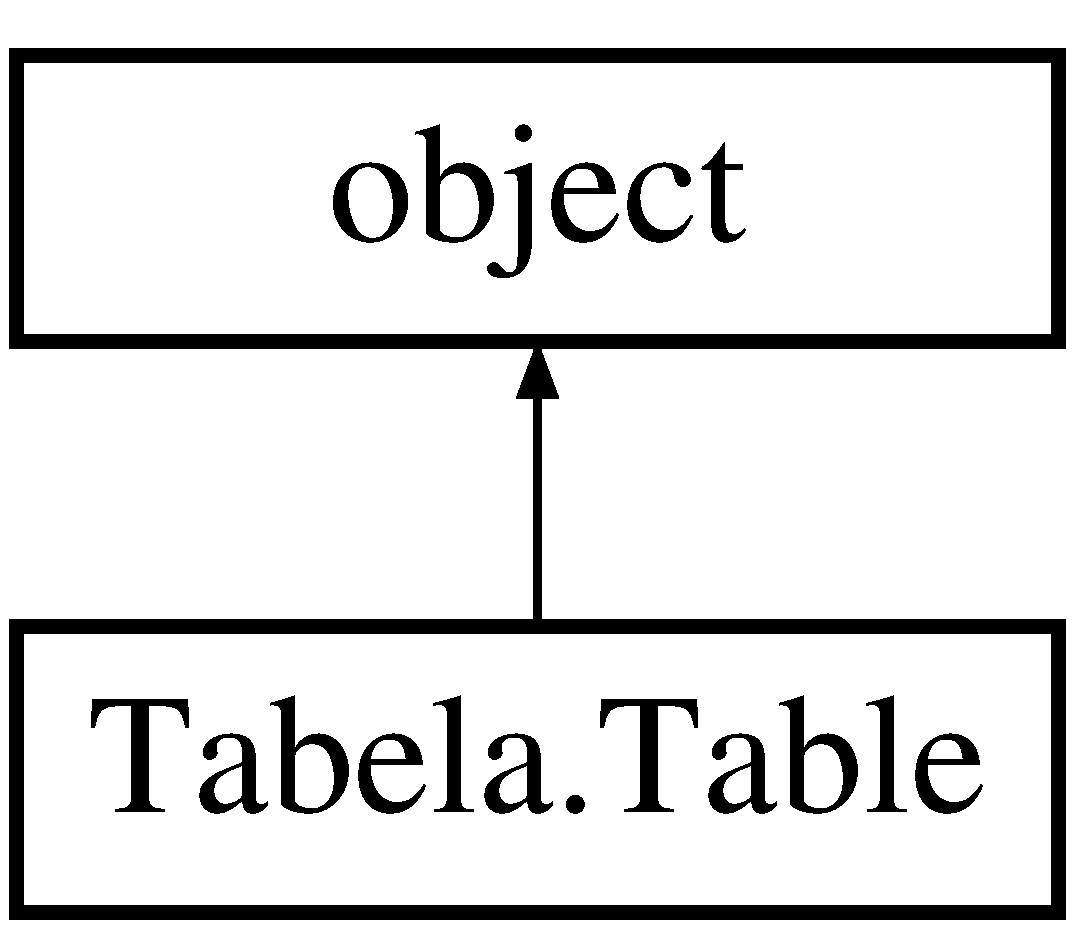
\includegraphics[height=2.000000cm]{class_tabela_1_1_table}
\end{center}
\end{figure}
\subsection*{Public Member Functions}
\begin{DoxyCompactItemize}
\item 
def \mbox{\hyperlink{class_tabela_1_1_table_a10c29642d83aa4daf8124db325f0a761}{\+\_\+\+\_\+init\+\_\+\+\_\+}} (self, raw\+\_\+table)
\end{DoxyCompactItemize}
\subsection*{Public Attributes}
\begin{DoxyCompactItemize}
\item 
\mbox{\Hypertarget{class_tabela_1_1_table_ab9ebb4ae6437d100c1ebdf046fa43bff}\label{class_tabela_1_1_table_ab9ebb4ae6437d100c1ebdf046fa43bff}} 
{\bfseries loc\+\_\+source}
\item 
\mbox{\Hypertarget{class_tabela_1_1_table_acf4034972f8ca45d84f255eee35be31d}\label{class_tabela_1_1_table_acf4034972f8ca45d84f255eee35be31d}} 
{\bfseries table\+\_\+label}
\item 
\mbox{\Hypertarget{class_tabela_1_1_table_a8f4f53b31818b05a2d512a4ffe670ed3}\label{class_tabela_1_1_table_a8f4f53b31818b05a2d512a4ffe670ed3}} 
{\bfseries table\+\_\+data}
\item 
\mbox{\Hypertarget{class_tabela_1_1_table_a6d45ff17a28fa07c40cebc2af231a645}\label{class_tabela_1_1_table_a6d45ff17a28fa07c40cebc2af231a645}} 
{\bfseries bound\+\_\+x}
\item 
\mbox{\Hypertarget{class_tabela_1_1_table_ac28a8176c31fa193847311967c5d993a}\label{class_tabela_1_1_table_ac28a8176c31fa193847311967c5d993a}} 
{\bfseries bound\+\_\+y}
\item 
\mbox{\Hypertarget{class_tabela_1_1_table_a38f8e9cd9b88c014664c0d908f8b931c}\label{class_tabela_1_1_table_a38f8e9cd9b88c014664c0d908f8b931c}} 
{\bfseries key\+\_\+cols}
\item 
\mbox{\Hypertarget{class_tabela_1_1_table_a8432925ee02ec678d2b2f823749c85bb}\label{class_tabela_1_1_table_a8432925ee02ec678d2b2f823749c85bb}} 
{\bfseries key\+\_\+row}
\item 
\mbox{\Hypertarget{class_tabela_1_1_table_a3528cb5d55a61bad4dba988b698445f2}\label{class_tabela_1_1_table_a3528cb5d55a61bad4dba988b698445f2}} 
{\bfseries keys}
\end{DoxyCompactItemize}


\subsection{Detailed Description}
\begin{DoxyVerb}Classe que representa uma tabela logica. Recebema uma Raw_Table e remove os campos desnecessarios Pode ser picklada\end{DoxyVerb}
 

\subsection{Constructor \& Destructor Documentation}
\mbox{\Hypertarget{class_tabela_1_1_table_a10c29642d83aa4daf8124db325f0a761}\label{class_tabela_1_1_table_a10c29642d83aa4daf8124db325f0a761}} 
\index{Tabela\+::\+Table@{Tabela\+::\+Table}!\+\_\+\+\_\+init\+\_\+\+\_\+@{\+\_\+\+\_\+init\+\_\+\+\_\+}}
\index{\+\_\+\+\_\+init\+\_\+\+\_\+@{\+\_\+\+\_\+init\+\_\+\+\_\+}!Tabela\+::\+Table@{Tabela\+::\+Table}}
\subsubsection{\texorpdfstring{\+\_\+\+\_\+init\+\_\+\+\_\+()}{\_\_init\_\_()}}
{\footnotesize\ttfamily def Tabela.\+Table.\+\_\+\+\_\+init\+\_\+\+\_\+ (\begin{DoxyParamCaption}\item[{}]{self,  }\item[{}]{raw\+\_\+table }\end{DoxyParamCaption})}

\begin{DoxyVerb}Inicializa Tabela com dados da raw table\end{DoxyVerb}
 

The documentation for this class was generated from the following file\+:\begin{DoxyCompactItemize}
\item 
C\+:/\+Users/\+P\+C/source/repos/\+Trabalho\+\_\+final\+\_\+cpd/\+Simple\+Graph\+No\+S\+Q\+L/Tabela.\+py\end{DoxyCompactItemize}

\hypertarget{class_trie_1_1_trie}{}\section{Trie.\+Trie Class Reference}
\label{class_trie_1_1_trie}\index{Trie.\+Trie@{Trie.\+Trie}}
Inheritance diagram for Trie.\+Trie\+:\begin{figure}[H]
\begin{center}
\leavevmode
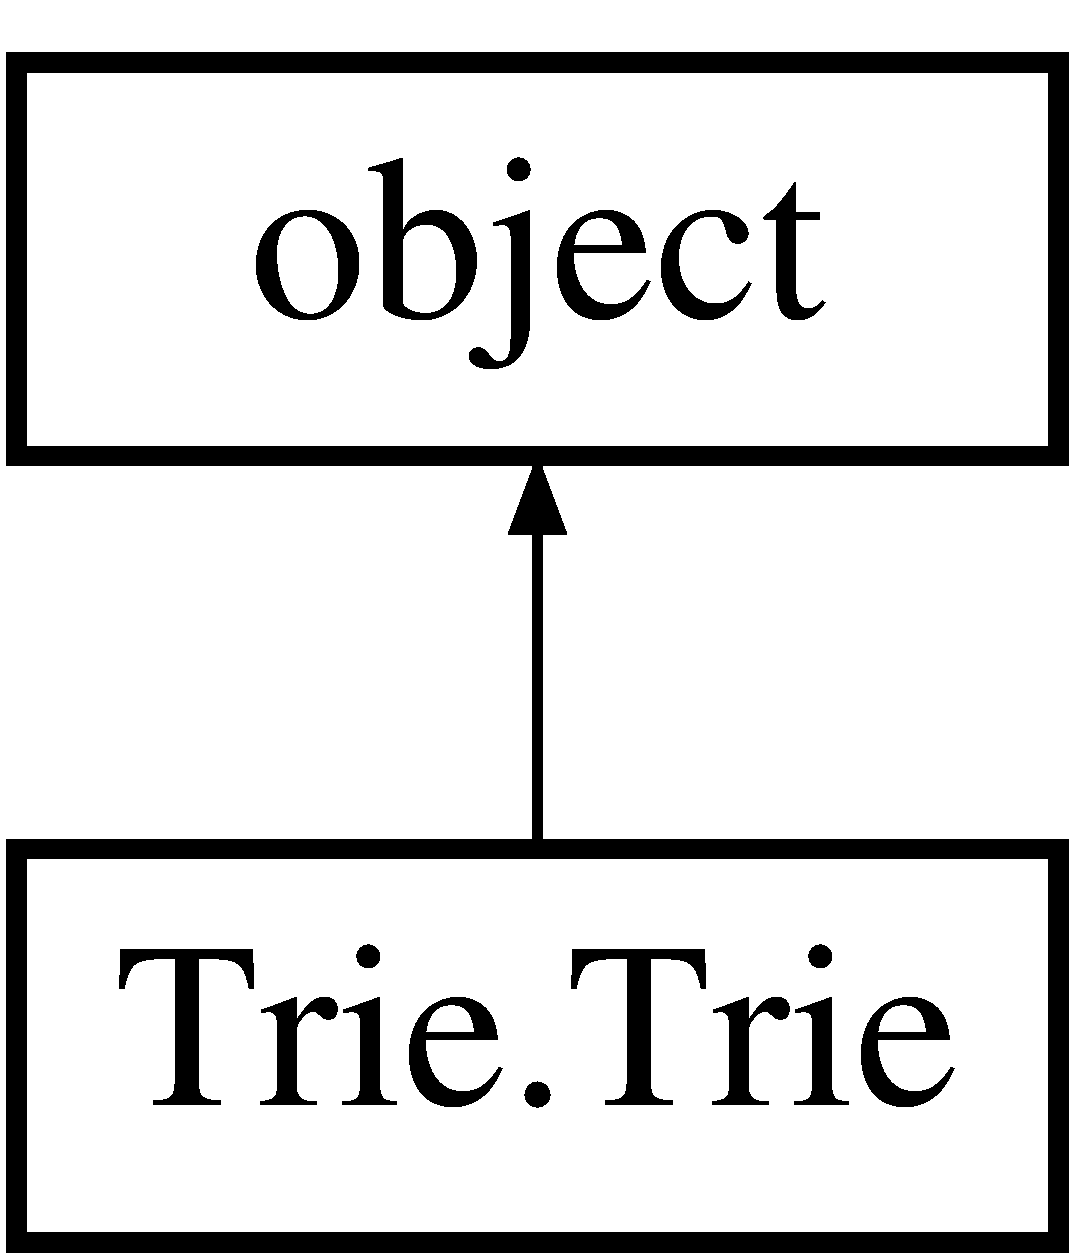
\includegraphics[height=2.000000cm]{class_trie_1_1_trie}
\end{center}
\end{figure}
\subsection*{Public Member Functions}
\begin{DoxyCompactItemize}
\item 
def \mbox{\hyperlink{class_trie_1_1_trie_a9b9de44cd1cfcf4001d34b1c435c0dd0}{\+\_\+\+\_\+init\+\_\+\+\_\+}} (self)
\item 
\mbox{\Hypertarget{class_trie_1_1_trie_a670d8832bdbe3b2f8f630188b4a3f997}\label{class_trie_1_1_trie_a670d8832bdbe3b2f8f630188b4a3f997}} 
def {\bfseries yield\+\_\+strings} (self, trie)
\end{DoxyCompactItemize}
\subsection*{Public Attributes}
\begin{DoxyCompactItemize}
\item 
\mbox{\Hypertarget{class_trie_1_1_trie_a323873a709ecdd62ebe123fa9c3abff4}\label{class_trie_1_1_trie_a323873a709ecdd62ebe123fa9c3abff4}} 
{\bfseries root}
\item 
\mbox{\Hypertarget{class_trie_1_1_trie_a83967a78c562d8aca0a9f979a14d6c98}\label{class_trie_1_1_trie_a83967a78c562d8aca0a9f979a14d6c98}} 
{\bfseries strings\+\_\+dict}
\item 
\mbox{\Hypertarget{class_trie_1_1_trie_aa4cff19308fc0f8647bd6b3fd06fc1af}\label{class_trie_1_1_trie_aa4cff19308fc0f8647bd6b3fd06fc1af}} 
{\bfseries strings\+\_\+list}
\item 
\mbox{\Hypertarget{class_trie_1_1_trie_acfbb76a3f77a007fbef4f7e270842f64}\label{class_trie_1_1_trie_acfbb76a3f77a007fbef4f7e270842f64}} 
{\bfseries reverse}
\end{DoxyCompactItemize}


\subsection{Detailed Description}
\begin{DoxyVerb}Implementa uma Trie para pesquisa no nome de tabelas de maneira eficiente\end{DoxyVerb}
 

\subsection{Constructor \& Destructor Documentation}
\mbox{\Hypertarget{class_trie_1_1_trie_a9b9de44cd1cfcf4001d34b1c435c0dd0}\label{class_trie_1_1_trie_a9b9de44cd1cfcf4001d34b1c435c0dd0}} 
\index{Trie\+::\+Trie@{Trie\+::\+Trie}!\+\_\+\+\_\+init\+\_\+\+\_\+@{\+\_\+\+\_\+init\+\_\+\+\_\+}}
\index{\+\_\+\+\_\+init\+\_\+\+\_\+@{\+\_\+\+\_\+init\+\_\+\+\_\+}!Trie\+::\+Trie@{Trie\+::\+Trie}}
\subsubsection{\texorpdfstring{\+\_\+\+\_\+init\+\_\+\+\_\+()}{\_\_init\_\_()}}
{\footnotesize\ttfamily def Trie.\+Trie.\+\_\+\+\_\+init\+\_\+\+\_\+ (\begin{DoxyParamCaption}\item[{}]{self }\end{DoxyParamCaption})}

\begin{DoxyVerb}Inicializa raiz da trie como um defaultdict com uma factory de dicionarios\end{DoxyVerb}
 

The documentation for this class was generated from the following file\+:\begin{DoxyCompactItemize}
\item 
C\+:/\+Users/\+P\+C/source/repos/\+Trabalho\+\_\+final\+\_\+cpd/\+Simple\+Graph\+No\+S\+Q\+L/Trie.\+py\end{DoxyCompactItemize}

%--- End generated contents ---

% Index
\backmatter
\newpage
\phantomsection
\clearemptydoublepage
\addcontentsline{toc}{chapter}{Index}
\printindex

\end{document}
